\chapter{Design}
% Some Introduction

\section{High Level Design }

\begin{figure}[htbp]
	\centering
	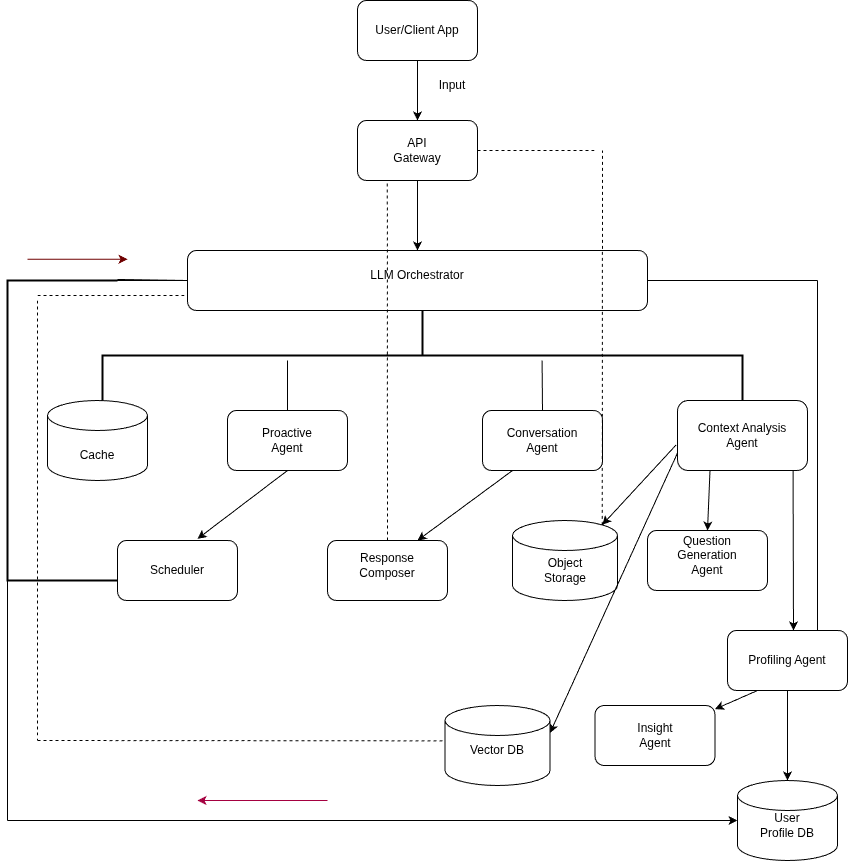
\includegraphics[scale=0.5]{design.png}
	\caption{High Level Design}
	\label{fig:high}
\end{figure}
	
\subsection{System Components}
\subsubsection{API Gateway}
Built using \texttt{FastAPI}, handling JWT authentication and serving as the interface for \textbf{Object Storage (S3)} uploads.

\subsubsection{LLM Orchestrator}
Implemented using \texttt{LangGraph} to manage state across specialized agents, utilizing \textbf{Redis} for Short-Term Memory (STM).

\subsubsection{Specialized Agents}
\begin{itemize}
	\item \textbf{Profiling Agent (PA):} Updates the \textbf{User Profile DB} with learner traits.
	\item \textbf{Content Analysis Agent (CAA):} Parses documents and stores embeddings in the \textbf{Vector DB}.
	\item \textbf{Question Generation Agent (QGA):} Creates assessments based on VDB context.
\end{itemize}

\section{Data Layer}
The system uses \textbf{PostgreSQL} for persistent profiles, \textbf{Pinecone} for semantic search, and \textbf{Redis} for session caching.

\section{System Architecture }

\begin{figure}[htbp]
	\centering
	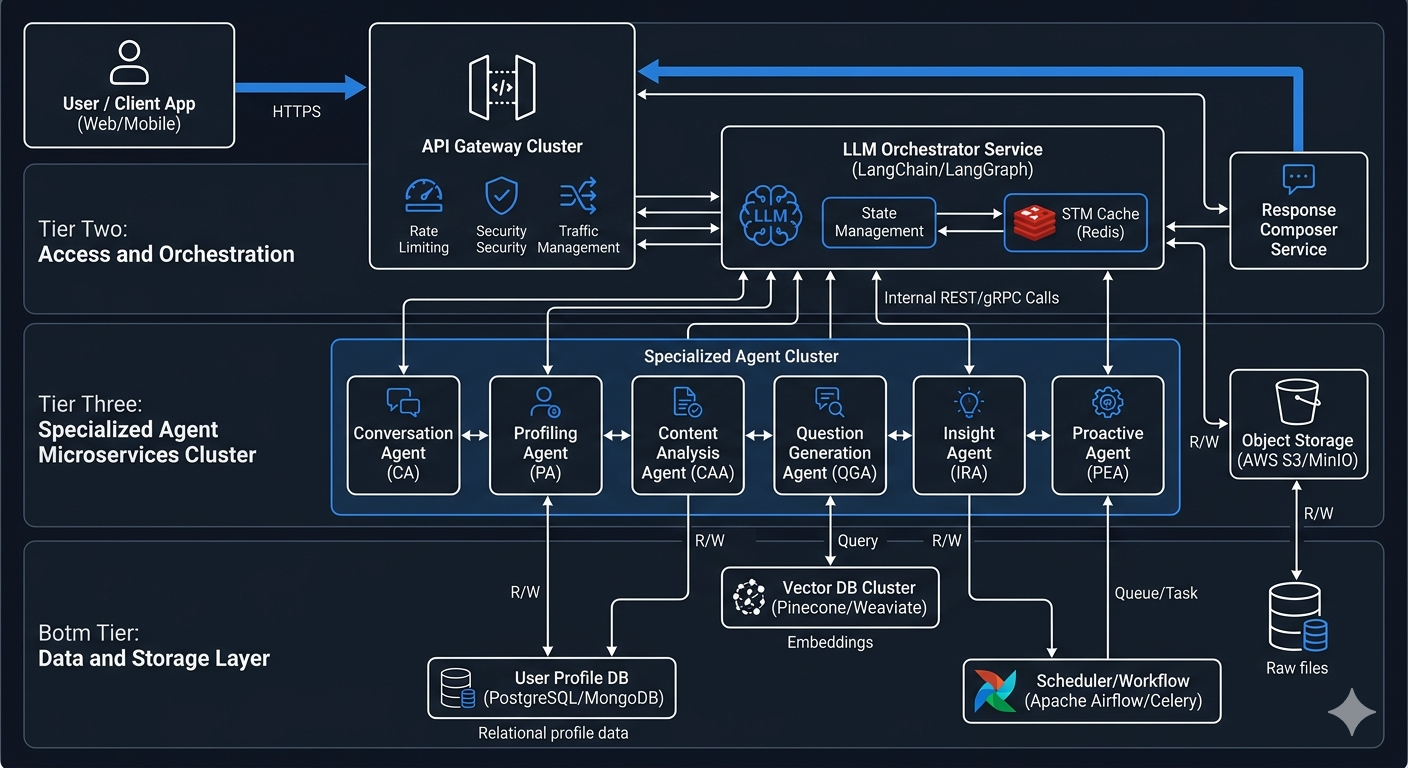
\includegraphics[scale=0.25]{arch.png}
	\caption{System Architecture}
	\label{fig:arch}
\end{figure}

%\section{Use-case Diagram }

%\section{Class Diagram}

%\section{Sequence Diagram}
%Include the Sequence diagram with respect to your project work